\section{Benzene Ring}

\begin{itemize}
    \item PPP- Model $U_{ij} = \frac{U_{ii}}{\sqrt{1+\alpha |d_i - d_j|^2}}$
    \item Hartree Term needed to shift Benzene spectrum
    \item compare PPP Benzene spectrum to Hörbinger Paper
    \item mention problem with pulse direction because benzene is just chain with PBC
    \item Hoppings are not time dependent since we say laser pulse only hits QD
\end{itemize}


%%%%%%%%%%%%%%%%%%%%%%%%%%%%%%%%%%%%%%%%%%%%%%%%%%%%%%%%%%%%%%%%%%%%%%%%%%%%%%%%%%

\subsection{Pariser-Parr-Pople Model}
The Pariser-Parr-Pople model (PPP) allows the Hamiltonian of single band $\pi$- electron systems with nearest neighbour hoppings to be simplified into a diagonalisable form.

\begin{equation}
    \mathcal{H}_{PPP} = \underbrace{-t \sum_{\langle ij \rangle \sigma} \left(\hat{c}^\dagger_{i\sigma}\hat{c}_{j\sigma} + h.c.\right) 
    }_{\text{hopping terms}}
    + \underbrace{U \sum_i \left(\hat{n}_{i\uparrow} - \frac{1}{2}\right)\left(\hat{n}_{i\downarrow} - {1\over 2}\right)
    }_{\text{local coulomb interaction}}
    + \underbrace{\frac{1}{2}\sum_{ij} U_{ij} \bigg(\hat{n}_{i} - 1\bigg)\bigg(\hat{n}_{i} - 1\bigg)
    }_{\text{non-Local Coulomb interactions}}
\end{equation}
Here $\langle \cdot\cdot\cdot \rangle$ indicates nearest neighbour hoppings and $\hat{n}_i = \hat{n}_{i\uparrow} + \hat{n}_{i\downarrow}$
\\

{\color{red} Q: We do not use this form in the code... instead we simply add $U$ and $U_{ij}$ wherever there is an interaction present... and on top of that we have an on-site hopping term a Hartree term... How would I write about this? Also Paul had a derivation of this Hartree term using some Feynmann diagram stuff... Should I write about that?}
\\

We model the energy of the non-local coulomb interaction using the Ohno parametrisation of the coulomb interaction  \cite{ppp_ohno, hoerbinger}
\begin{equation}
    U_{ij} = \frac{U}{\sqrt{1 + \alpha |r_{ij}|^2}} \quad \text{where} \quad \alpha = \left(\frac{4\pi\varepsilon_0 U}{e^2} \right)^2 \label{eq:ohno_interpolation}
\end{equation}
where $|r_{ij}|$ is the distance between two sites. This ensures that at long ranges, $r_{ij}\to\infty$, $U_{ij}$ gives the standard Coulomb interaction energy, and at short ranges, $r_{ij}\to 0$, we get the on-site coulomb interaction $U_{ij} = U_{ii} =: U$ 

\subsection{Hexagonal Geometry}

We model the Benzene ring as a 6-site chain with periodic boundary conditions. This has the benefit that it is simple to implement in the existing framework, as a 6x1 lattice with a hopping between sites $0$ and $5$. However, in doing so we loose the orientation of the lines connecting two sites, relative to the laser pulse. {\color{red} This leads to an inaccuracy in the time dependence of the hoppings between the sites. But it is small?}
\begin{figure}[!hbt]
    \centering
    \begin{tikzpicture}[decoration=snake,
                    Benzene/.style={draw,thick, circle, radius = .1em, fill=red!80!yellow},
                    squiggly/.style={->, decorate, thick, yellow!70!red},
                    doublearrow/.style={->, double, line width=1pt, -Implies, double distance=3pt, shorten >= 2cm, shorten <=2cm}
                    ]
    % RING %
    \newdimen\R
    \R=1.5cm
    \draw[thick] (0:\R)
    \foreach \x in {60,120,...,360} {  -- (\x:\R) }
    -- cycle (360:\R) node[Benzene, label=3] (Bc3){}
    -- cycle (300:\R) node[Benzene, label=4] (Bc4){}
    -- cycle (240:\R) node[Benzene, label=5] (Bc5){}
    -- cycle (180:\R) node[Benzene, label=0] (Bc0){}
    -- cycle (120:\R) node[Benzene, label=1] (Bc1){}
    -- cycle  (60:\R) node[Benzene, label=2] (Bc2){};
    
    \foreach \x in {0,1,2,3,4,5}{
    \draw[squiggly] ($(Bc\x) + (-1, 1)$) -- (Bc\x);
    }
    
    % CHAIN DOWN%
    \foreach \x in {0,1,2,3,4,5}{
    \node[Benzene, label=below:\x] at ($(1.3*\x,0) + (7,-1.3)$)  (B\x){};
    \draw[squiggly] ($(B\x) + (-1, 1)$) -- (B\x);
    }
    
    \foreach \x/\y in {0/1,1/2,2/3,3/4,4/5}{
    \draw[thick] (B\x) -- (B\y);
    }
    \draw[dashed] ($(B0) - (0.7,0)$) -- (B0);
    \draw[dashed] (B5) -- ($(B5) + (0.7,0)$);
    
    % CHAIN UP %
    \foreach \x in {0,1,2,3,4,5}
    \node[Benzene, label=below:\x] at ($(1.3*\x,0) + (7,1.3)$)  (Bu\x){};
    
    \foreach \x/\angle in {0/80, 1/135, 2/190, 3/260, 4/340, 5/20}
    \draw[squiggly] ($(Bu\x) + (\angle:1.4)$) -- (Bu\x);
    
    \foreach \x/\y in {0/1,1/2,2/3,3/4,4/5}
    \draw[thick] (Bu\x) -- (Bu\y);
    
    \draw[dashed] ($(Bu0) - (0.7,0)$) -- (Bu0);
    \draw[dashed] (Bu5) -- ($(Bu5) + (0.7,0)$);
    
    % DOUBLE ARROWS %
    \draw[doublearrow] (Bc3) -- (Bu0) node[pos=0.5,sloped,rotate=150]{\color{red}\Huge$|$}node[pos=0.5,rotate=40]{\color{red}\Huge$|$};;
    \draw[doublearrow] (Bc3) -- (B0);
    
    \end{tikzpicture}
    \caption{Caption}
\end{figure}

    %%%%%%%%%%%%%%%%%
    % PULSE ON LINE %
    %%%%%%%%%%%%%%%%%
    
\begin{figure}[!hbt]
    \centering
    \begin{tikzpicture}[decoration=snake,
                    Benzene/.style={draw,thick, circle, radius = .1em, fill=red!80!yellow},
                    squiggly/.style={->, decorate, thick, yellow!70!red},
                    doublearrow/.style={->, double, line width=1pt, -Implies, double distance=3pt, shorten >= 2cm, shorten <=2cm}
                    ]
                    
    
    % RING %
    \foreach \x/\y in {0/1,1/2,2/3,3/4,4/5,5/0}{
    \draw[squiggly] ($(Bc\x)!0.5!(Bc\y) + (-1,1)$) -- ($(Bc\x)!0.5!(Bc\y)$);
    }
    \newdimen\R
    \R=1.5cm
    \draw[thick] (0:\R)
    \foreach \x in {60,120,...,360} {  -- (\x:\R) }
    -- cycle (360:\R) node[Benzene, label=3] (Bc3){}
    -- cycle (300:\R) node[Benzene, label=4] (Bc4){}
    -- cycle (240:\R) node[Benzene, label=5] (Bc5){}
    -- cycle (180:\R) node[Benzene, label=0] (Bc0){}
    -- cycle (120:\R) node[Benzene, label=1] (Bc1){}
    -- cycle  (60:\R) node[Benzene, label=2] (Bc2){};
    
    
    % CHAIN DOWN%
    \foreach \x in {0,1,2,3,4,5}
    \node[Benzene, label=below:\x] at ($(1.3*\x,0) + (7,-1.3)$)  (B\x){};
    
    \foreach \x/\y in {0/1, 1/2, 2/3, 3/4, 4/5}
    \draw[squiggly] ($(B\x)!0.5!(B\y) + (-1, 1)$) -- ($(B\x)!0.5!(B\y)$);
    
    \foreach \x/\y in {0/1,1/2,2/3,3/4,4/5}
    \draw[thick] (B\x) -- (B\y);
    
    \draw[dashed] ($(B0) - (0.7,0)$) -- (B0);
    \draw[dashed] (B5) -- ($(B5) + (0.7,0)$);
    
    % CHAIN UP %
    \foreach \x/\y/\angle in {0/1/80, 1/2/135, 2/3/190, 3/4/260, 4/5/340}
    \draw[squiggly] ($(Bu\x)!0.5!(Bu\y) + (\angle:1.4)$) -- ($(Bu\x)!0.5!(Bu\y)$);
    
    \foreach \x in {0,1,2,3,4,5}
    \node[Benzene, label=below:\x] at ($(1.3*\x,0) + (7,1.3)$)  (Bu\x){};

    \foreach \x/\y in {0/1,1/2,2/3,3/4,4/5}
    \draw[thick] (Bu\x) -- (Bu\y);

    \draw[dashed] ($(Bu0) - (0.7,0)$) -- (Bu0);
    \draw[dashed] (Bu5) -- ($(Bu5) + (0.7,0)$);
    

    % DOUBLE ARROWS %
    \draw[doublearrow] (Bc3) -- (Bu0) node[pos=0.5,sloped,rotate=150]{\color{red}\Huge$|$}node[pos=0.5,rotate=40]{\color{red}\Huge$|$};
    \draw[doublearrow] (Bc3) -- (B0);
    \end{tikzpicture}
    \caption{Caption}
\end{figure}

The C-C bond length in bezene is $\SI{1.40}{\angstrom}$. This together with the hexagonal geometry allows us to determine $U_{ij}$ (\ref{eq:ohno_interpolation}) 

\begin{figure}[!hbt]
    \centering
    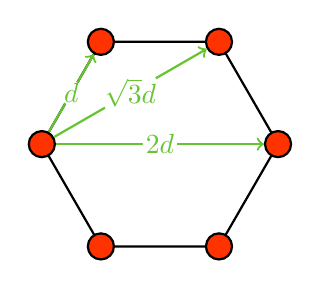
\begin{tikzpicture}[Benzene/.style={draw,thick, circle, radius = .1em,                                      fill=red!80!yellow},
                    arrow/.style={->, thick, yellow!40!green},
                    arrow_label/.style={midway, circle, fill=white, inner sep=0}
                    ]
        \newdimen\R
        \R=1.5cm
        \draw[thick] (0:\R)
        \foreach \x in {60,120,...,360} {  -- (\x:\R) }
        -- cycle (360:\R) node[Benzene] (Bc3){}
        -- cycle (300:\R) node[Benzene] (Bc4){}
        -- cycle (240:\R) node[Benzene] (Bc5){}
        -- cycle (180:\R) node[Benzene] (Bc0){}
        -- cycle (120:\R) node[Benzene] (Bc1){}
        -- cycle  (60:\R) node[Benzene] (Bc2){};
        
        \draw[arrow] (Bc0) -- (Bc1) node[arrow_label] {$d$};
        \draw[arrow] (Bc0) -- (Bc2) node[arrow_label] {$\sqrt{3}d$};
        \draw[arrow] (Bc0) -- (Bc3) node[arrow_label] {$2d$};
    \end{tikzpicture}
    \caption{Interatomic distances in Benzene ($d=\SI{1.40}{\angstrom})$}
\end{figure}


